\documentclass[12pt]{article}
\usepackage[left=1in, right=1in, top=1in,bottom = 1in]{geometry}
\usepackage{amsmath}
\usepackage{xcolor}
\usepackage{lmodern}
\usepackage{listings}
\usepackage{graphicx}
\usepackage{float}
\usepackage{fancyhdr}
\usepackage{lastpage}
\usepackage{subfig}
\usepackage{hyperref}
\definecolor{backcolour}{rgb}{0.95,0.95,0.92}

\pagestyle{fancy}
\fancyhf{}
\rhead{Max Le}
\lhead{FINAL PROJECT}
\cfoot{\thepage\ of \pageref{LastPage}}

\lstset{language=[90]Fortran,
  backgroundcolor=\color{backcolour},   
  basicstyle=\ttfamily,
  keywordstyle=\color{red},
  commentstyle=\color{blue},
  showstringspaces=false,
  morecomment=[l]{!\ }% Comment only with space after !
}



\begin{document}
	\begin{flushleft}
		Max Le \\
		ID: 901223283\\
		Introduction To Parallel Process\\
        Final Project: Parallelization Of 1D Shocktube 
    \end{flushleft}

    \tableofcontents
    \newpage

    \section{INTRODUCTION}

    The aim of this project is to parallelize a 1-D shocktube.  In compressible aerodynamics, shock waves are detrimental to the performance of aircraft; especially when we are going much faster than the speed of sound (supersonic). In order to simplify things, we are going to assume the following: 

    \begin{itemize}
        \item problem is 1D
        \item affects of heat transfer or external forces are negligible 
        \item ideal gas and single phase
        \item boundary conditions are zero gradient, so that we are only interested in how the shock propagates.         
    \end{itemize}
    \noindent
    This problem is governed by a set of hyberbolic PDEs, which represent the conservation of mass, momentum and energy: 
    
    \begin{equation}
        \begin{aligned}
            &\dfrac{\partial \rho}{\partial t} + \dfrac{\partial \rho u }{\partial x} = 0 \\ \\ 
            &\dfrac{\partial \rho u}{\partial t} + \dfrac{\partial (p+\rho u^2)) }{\partial x} = 0 \\ \\ 
            &\dfrac{\partial E}{\partial t} + \dfrac{\partial (E+p)u }{\partial x} = 0
        \end{aligned}        
    \end{equation}

    \noindent
    where $\rho$, $u$, $p$, and $E$ are density, velocity, pressure and total energy respectively. In a compact form, these equations can then be written as:

    \begin{equation}
        \begin{aligned}
            &\dfrac{\partial U}{\partial t} + \dfrac{\partial F(U)}{\partial x} = 0, \text{ where}\\
            U&= \begin{bmatrix}
                \rho\\
                \rho u \\
                E
            \end{bmatrix} \\
            F&= \begin{bmatrix}
                \rho u \\
                p + \rho u^2\\
                (E+p)u                
            \end{bmatrix}        
        \end{aligned}
    \end{equation}

    \newpage
    The shocktube looks something like this at initial time: 

    \begin{figure}[H]
        \begin{center}
        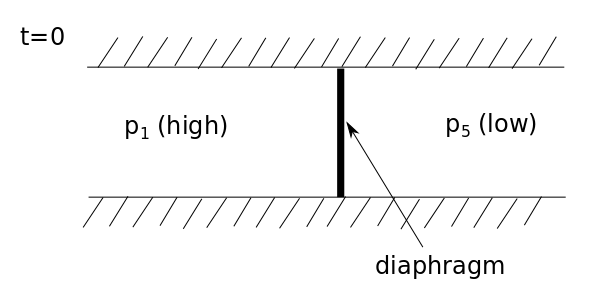
\includegraphics[height = 40mm,width = 80mm]{IC_sod.png}
        \caption{The shocktube at t = 0}
        \end{center}
    \end{figure}     

    \noindent
    The basic idea is that we are going to set the left and right chamber in the shocktube at different pressure and densities.  Then, once the diaphragm is removed, we will have a shockwave propagating from the higher pressure region into the lower pressure region.  At the same time, we would also see an expansion fan going in the opposite direction. In order to make things simpler, our shocktube's length is from -10 m to 10 m and the location of the diaphgram is at 0 m. The initial data for both chambers are:

    \begin{align*}
        P_L &= 1.00 \\
        P_R &= 0.125 \\
        \rho_L &= \dfrac{1.00}{\gamma -1} \\
        \rho_R &= \dfrac{0.125}{\gamma-1}\\
        U_L &= U_R = 0.0
    \end{align*}


    \begin{figure}[H]
        \begin{center}
        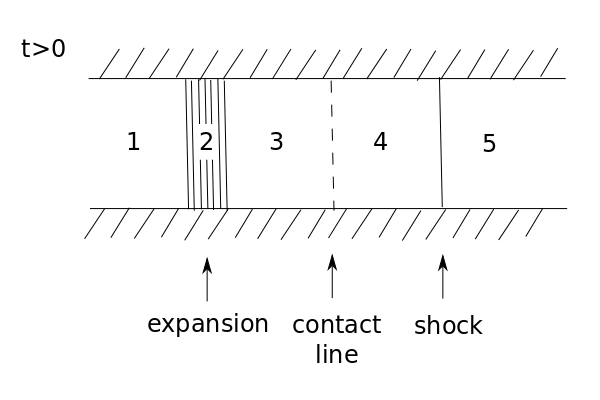
\includegraphics[height = 40mm,width = 80mm]{solution_sod.png}
        \caption{The shocktube as t $>$ 0}
        \end{center}
    \end{figure}  

    \newpage
    \section{NUMERICAL METHODS}

    \subsection{Discretizations}
    We are going to employ a first order scheme to solve this problem. Specifically, the temporal derivative is discretized as a first order forward in time, while the spatial derivatives are discretized as first order in space.  For the spatial terms, the sign of the speed of sound will dictate whether we should use first order forward or first order backward (upwind and downwind).  Generally, the discretization looks like this: 

    \begin{equation}
        \begin{aligned}
            &\dfrac{\partial U}{\partial t} \approx \dfrac{U^{n+1}_i-U^n_i}{\Delta t} + \mathcal{O}(\Delta t)\\ \\
            &\dfrac{\partial F}{\partial x} \approx \dfrac{F^{n}_{i+1}-F^n_i}{\Delta x} + \mathcal{O}(\Delta x)
        \end{aligned}        
    \end{equation}

    \noindent
    Together, we can write our finite difference equation for this scheme as follow: 

    \begin{equation}
        U^{n+1}_{i} = U_i^n-\dfrac{\Delta t}{\Delta x}\left[(F^+ + F^-)_{i+1/2}-(F^+ + F^-)_{i-1/2}\right]
    \end{equation}
    \subsection{Computational grid}
    \noindent
    It should be noted that $F^+$ and $F^-$ stand for positive and negative fluxes respectively.  For a given edge, say at $i-\dfrac{1}{2}$, there will be both positive and negative fluxes.  
    \noindent \newline
    Our grid for this finite volume method will be a cell centered grid, where U is defined at the center and the fluxes are defined on the edges. 

    \begin{figure}[H]
        \begin{center}
        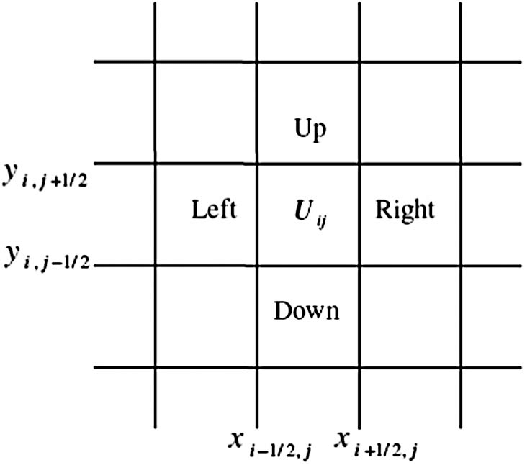
\includegraphics[height = 40mm,width = 80mm]{grid.png}
        \caption{Finite volume grid}
        \end{center}
    \end{figure}

    \noindent
    In order to retain numerical stability, we would calculate our timestep as follow and the minimum timestep will be chosen: 

    \begin{equation}
        dt = \dfrac{CFL*dx}{|u|+a}
    \end{equation}

    \noindent
    \subsection{Fluxes}
    The fluxes are computed as Van Leer fluxes for its simpliicty and ability to handle both subsonic as well as supersonic case. Denote the local mach number as "M" and the speed of sound as "a", the Van Leer fluxes are as follow for both positive and negative fluxes: 


    \begin{align}
        \vec{F}^{\pm} &= \begin{bmatrix}
               f_a^{\pm} \\
               f_a^{\pm}f_b^{\pm}\dfrac{1}{\gamma} \\
               f_a^{\pm}f_b^{\pm}f_b^{\pm} \dfrac{1}{2(\gamma^2-1)}
             \end{bmatrix}
      \end{align}

      \noindent
      where $f_a$ and $f_b$ are as follow: 

      \begin{align*}
          f_a^{\pm} &= \pm \dfrac{1}{4}\rho a (M\pm 1)^2\\
          f_b^{\pm} &= \pm (\gamma -1)M a \pm 2a
      \end{align*}


    \newpage
    \section{PARALLELIZATION STRATEGY}

    In order to parallelize this problem, we are going to use MPI to split up the arrays into chunks.  Each chunk will be processed by each processor.  Again, to keep this simple, we are going to assume that the number of processors is divisible by the array's length. This is done so that we only get whole number when calculate the local indices. 
    
    \begin{figure}[H]
        \begin{center}
        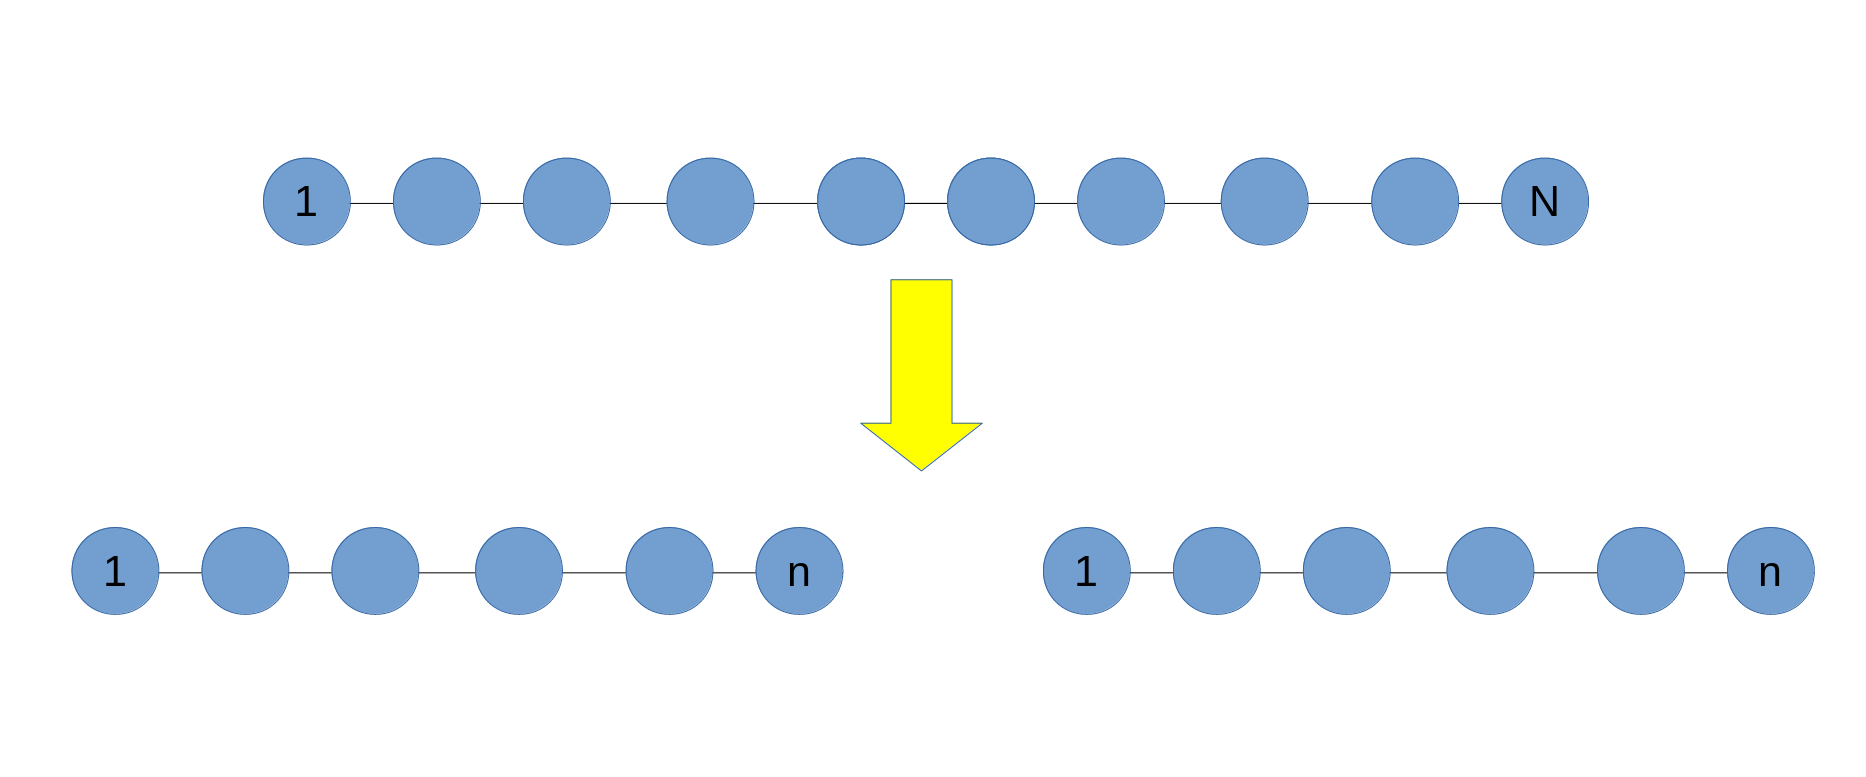
\includegraphics[height = 40mm,width = 100mm]{split.png}              
        \caption{Splitting of the main arrays}
        \end{center}  
    \end{figure}
    
    \noindent
    The local indices are calculated as follow. Because Fortran starts at 1, so we have 101 data points; then the last processor will be 1 data point shorter. Therefore, we added 1 point if it is the last processor. 

    \begin{lstlisting}
    nblocks = FLOOR(REAL(IMAX/nprocs))
    rem = IMAX - nblocks*nprocs
    !! Real start index on each chunk
    iStart = (nblocks*rank) + ghostPoints       

    localLOW = 1+ghostPoints
    localHIGH = nblocks+ghostPoints
    maxLocal = localHIGH + ghostPoints
    minLocal = localLOW-ghostPoints

    !! adding the remaining point
    if(rem /= 0) then
        if(rank == nprocs-1) then
            localHIGH = localHIGH + 1
            maxlocal  = maxlocal + 1
        end if
    end if

    \end{lstlisting}
    
    \noindent
    The current numerical scheme that we are using is a first order scheme; therefore, we would need data from left or right neighbor to update the boundaries.  As a result, ghost points are added and then they are exchanged across the boundaries using MPI Isend and MPI Irecv to avoid blocking communications.    

    \begin{figure}[H]
        \begin{center}
        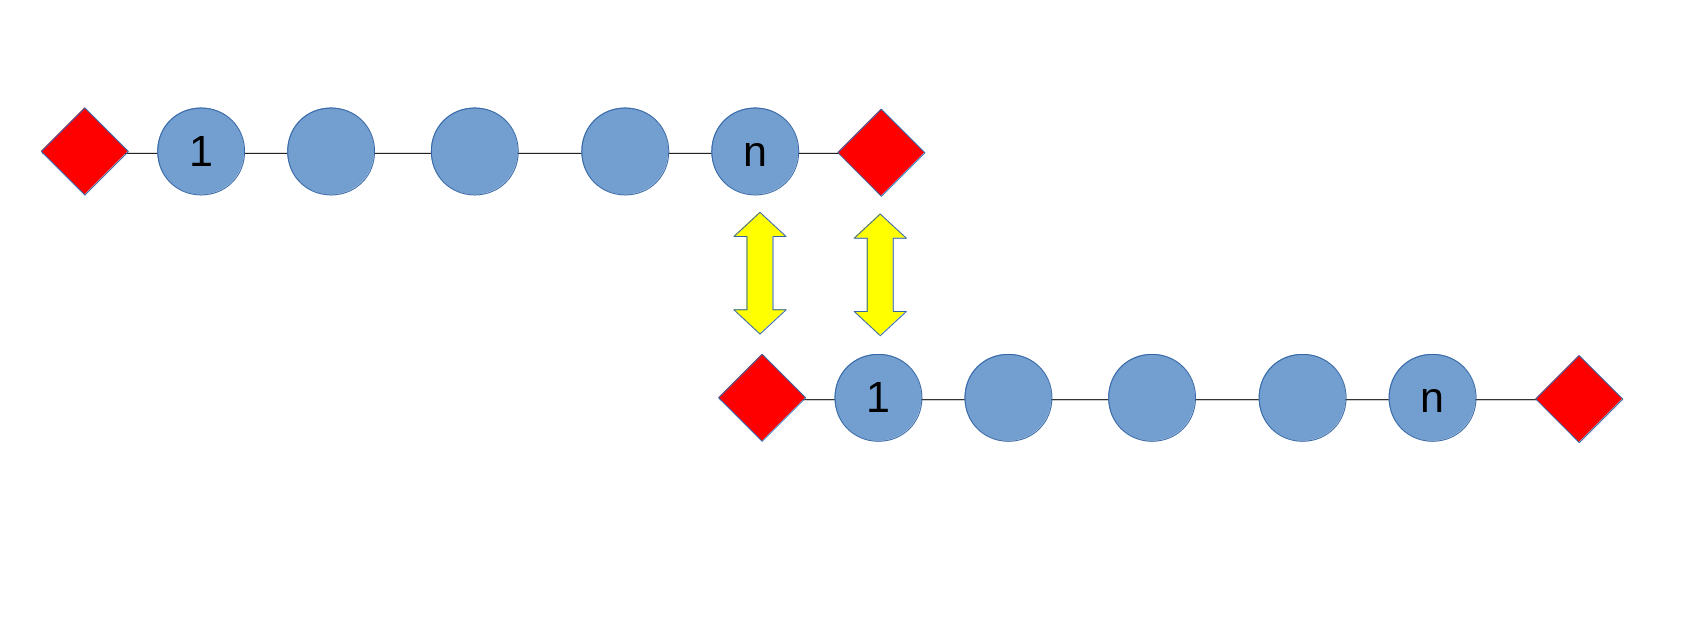
\includegraphics[height = 40mm,width = 100mm]{ghost.png}              
        \caption{Ghost points send/recv}
        \end{center}  
    \end{figure}       

    \noindent
    Furthermore, we can also optimize this by sending more ghost points.  The idea is that if more ghost points are sent; then the main solver should have enough data to keep updating the solutions without asking for more communications.  In other words, if 4 ghost points are sent; then for the next 4 timesteps, the code only needs to update the solution because it already has enough information (from 4 ghost points) to carry out the calculations. 

    \noindent \newline
    The way to implement this optimization is by using a flag in the update function. This flag will be set to the number of ghost points and send/recv are also done initially. Then everytime the code runs, this flag will decrease by 1 until it reaches zero and then it would be set to the number of ghost points again.  In code, this looks something like this: 
    
    \begin{lstlisting}
subroutine update2(temp) 
    include 'mpif.h' 
    use globalvar
    integer, intent(inout) :: temp 

    !! FLUX CALCULATIONS 
    do i = minLocal, maxLocal            
        
        call vanleer(fiph, fimh, state_vector, i, gamma)
        fGLOBALm(:,i) = fimh(:)
        fGLOBALp(:,i) = fiph(:)

    end do

    !! FINITE DIFFERENCE 
    do i = localLOW,localHIGH 
        do j=1,3
            U(j,i,2) = U(j,i,1)- (global_dt/dx)*&
            (fGLOBALp(j,i)-fGLOBALp(j,i-1))&
            - (global_dt/dx)*(fGLOBALm(j,i+1)&
            -fGLOBALm(j,i))
        end do
    end do
    if (temp == 0) then
        print*, "DOING SEND/RECV" 
        call bc_send 
        call bc_recv
        temp = ghostPoints 
    end if 
    temp = temp -1
    print*, "This is flag ", temp
    !! Update boundary 
    call boundary
end subroutine update2        
    \end{lstlisting}
    \newpage
    \section{RESULTS}

    \subsection{Numerical vs Analytical}
    Below is the comparison between the numerical and the analytical results. Excellent agreement is observed for a first order scheme. Although this is only valid for low pressure ratio. For higher pressure ratio, a higher order scheme is needed.  Please note that this analytical solution is not part of the project.  Its only purpose is to show that the results obtained are correct. The analytical solver was taken as a Python version of Dr. Timmes's Fortran code at Arizona State University.  This is reference in details later on. 



    \begin{figure}[H]
        \begin{center}
        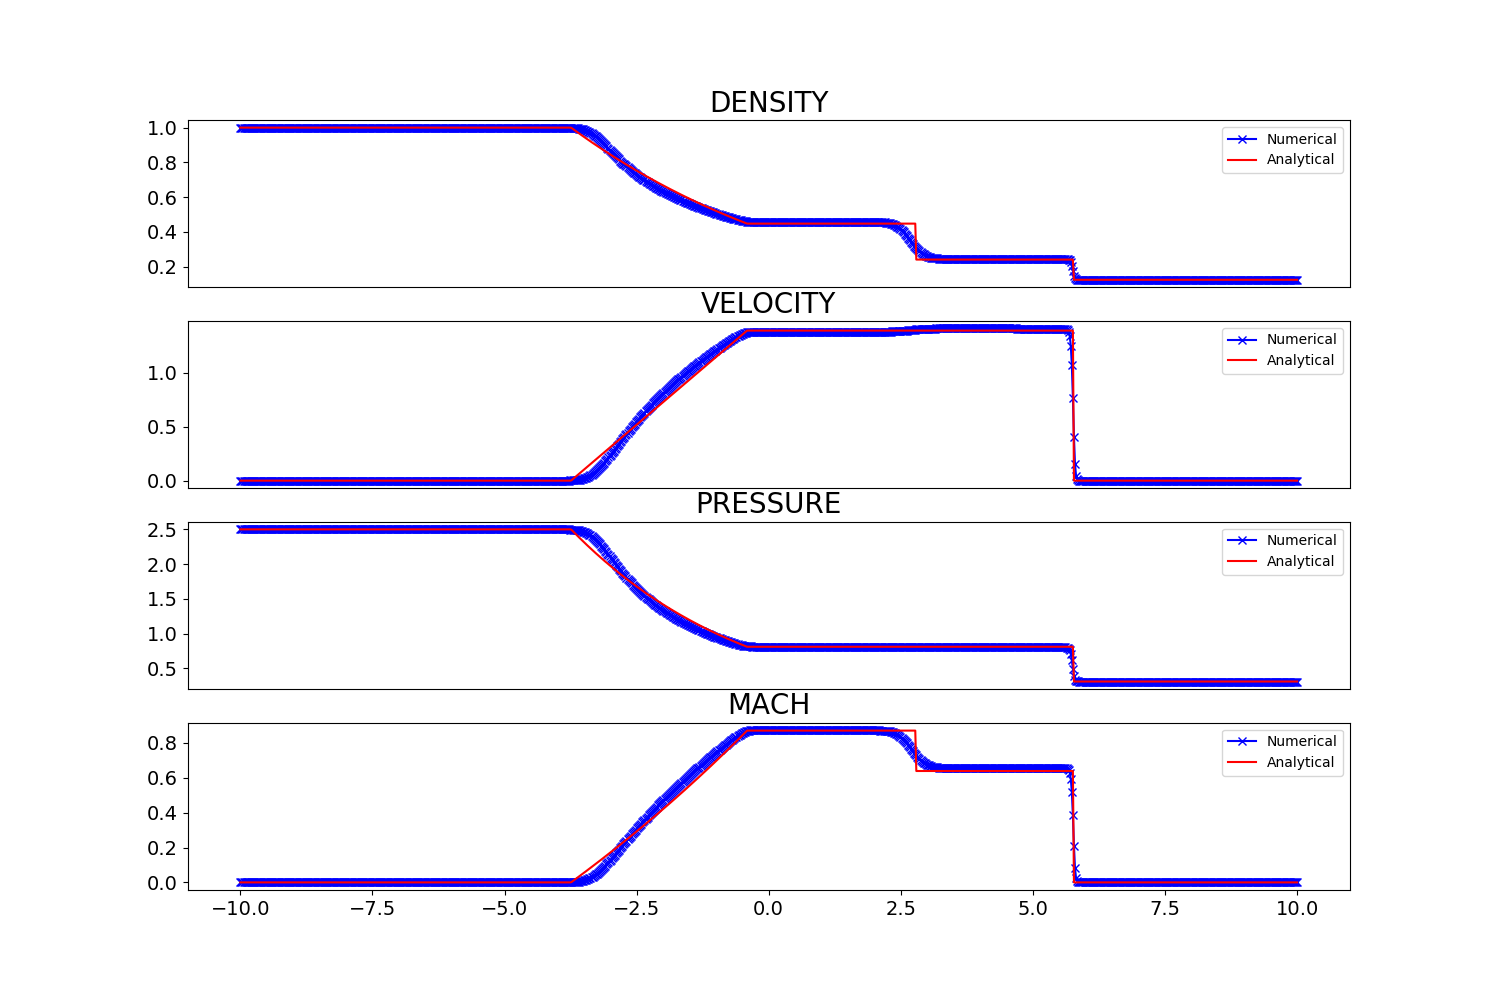
\includegraphics[height = 90mm,width = 160mm]{ana_num.png}              
        \caption{Analytical vs Numerical}
        \end{center}  
    \end{figure}    
    \noindent
    \subsection{Speedup}
    The code is timed using the "time" function in linux.  Blueshark runs a version of Linux distro so this method works. This is to prevent the hassle of putting everything back together in 1 giant array at the end. The output is done by having each processor appends out its own version of the array to a file. 
    Using Blueshark, the following speedup results are obtained for a problem size of \textbf{10,000} and \textbf{2 ghost points}. 

    \begin{figure}[H]
        \begin{center}
        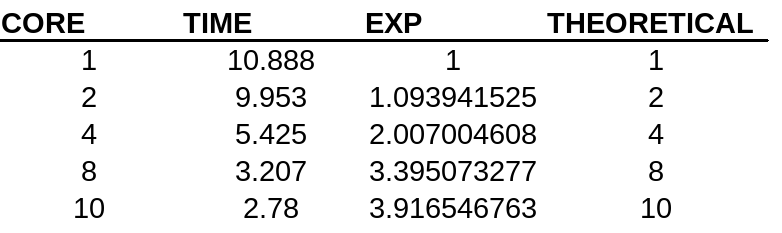
\includegraphics[height = 35mm,width = 100mm]{table_1g_speed.png}              
        \end{center}  
    \end{figure}       


    \begin{figure}[hbt!]
        \begin{center}
        \hspace*{2.5cm}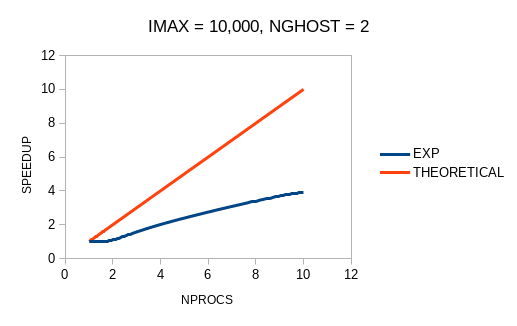
\includegraphics[height = 80mm,width = 140mm]{plot_1g_speed.png}
        \caption{Speedup for 2 ghost points}              
        \end{center}  
    \end{figure}    
    

    
    \newpage
    \noindent
    Also using Blueshark, the results are also obtained for a problem size of \textbf{10,000} and \textbf{10 ghost points}. 


    \begin{figure}[H]
        \begin{center}
        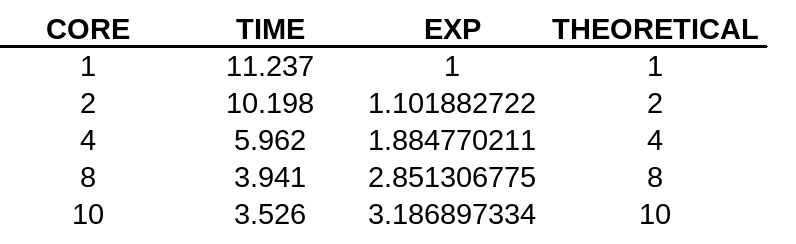
\includegraphics[height = 35mm,width = 100mm]{table_10g_speed.png}              
        \end{center}  
    \end{figure}       


    \begin{figure}[hbt!]
        \begin{center}
        \hspace*{2.5cm}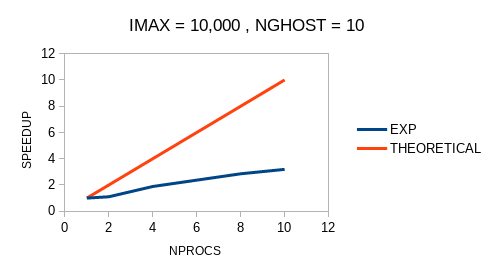
\includegraphics[height = 80mm,width = 140mm]{plot_10g_speed.png}   
        \caption{Speedup for 10 ghost points}                       
        \end{center}  
    \end{figure}    


    \newpage
    \noindent
    Effects of ghost points are investigated on smaller problem size

    \begin{figure}[H]
        \begin{center}
        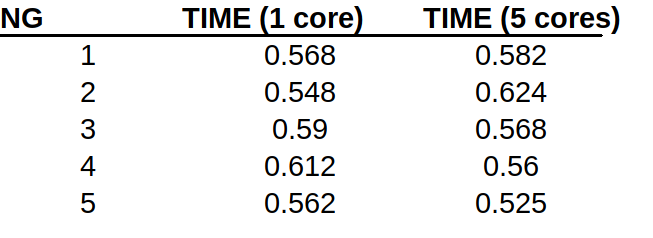
\includegraphics[height = 35mm,width = 100mm]{ghostInvest.png}              
        \end{center}  
    \end{figure}       


    \begin{figure}[H]
        \begin{center}
        \hspace*{2.5cm}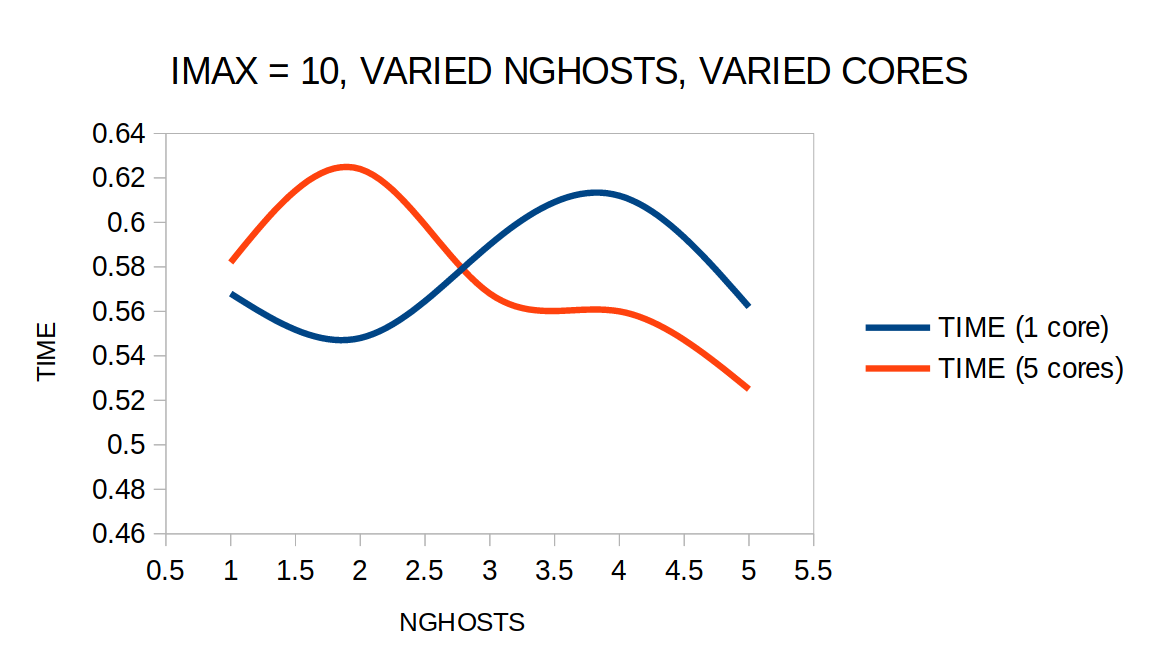
\includegraphics[height = 80mm,width = 140mm]{smallGhosts.png}
        \caption{IMAX = 10, varied ghost points and cores}                       
        \end{center}  
    \end{figure}    

    \newpage
    \subsection{Scalable}
    Regarding the scalability of the code, below are results for using Blueshark's "mpif.h" and the official MPI's "use mpi" for Fortran.  The problem size is \textbf{10,000} and the number of ghost points is kept at \textbf{2}. To do the scalability test, we assume problem size and number of core are related by a 1000:1 ratio. 

    \noindent
    \\
    Using Blueshark's mpif.h
    \begin{figure}[H]
        \begin{center}
        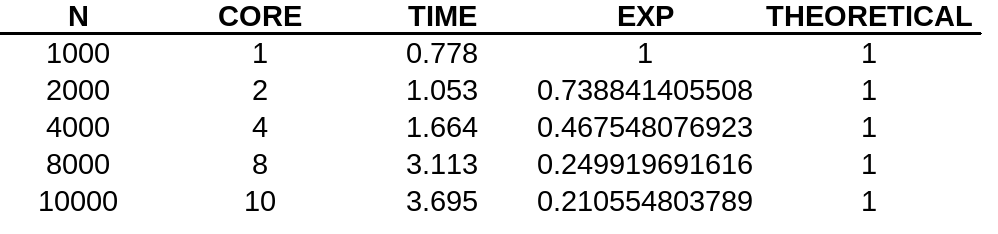
\includegraphics[height = 30mm,width = 100mm]{scaleBStable.png}             
        \end{center}  
    \end{figure}       


    \begin{figure}[H]
        \begin{center}
        \hspace*{2.5cm}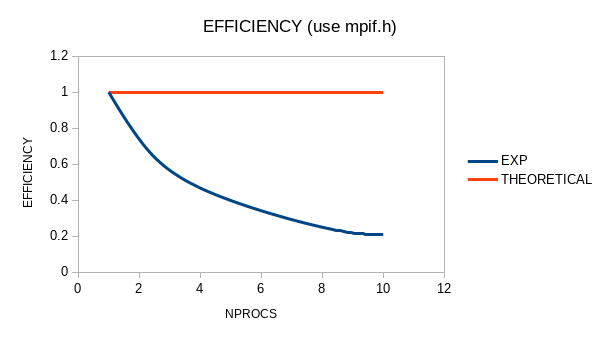
\includegraphics[height = 65mm,width = 140mm]{scaleBSplot.png}   
        \caption{Scaling for mpif.h}                       
        \end{center}  
    \end{figure}    

    \newpage
    \noindent
    Using the official MPI header
    \begin{figure}[H]
        \begin{center}
        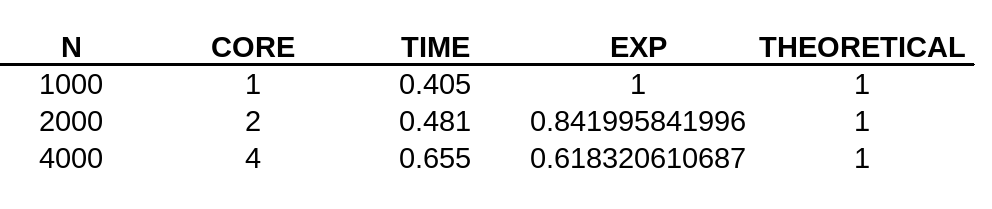
\includegraphics[height = 30mm,width = 100mm]{scaleMPItable.png}             
        \end{center}  
    \end{figure}       


    \begin{figure}[H]
        \begin{center}
        \hspace*{2.5cm}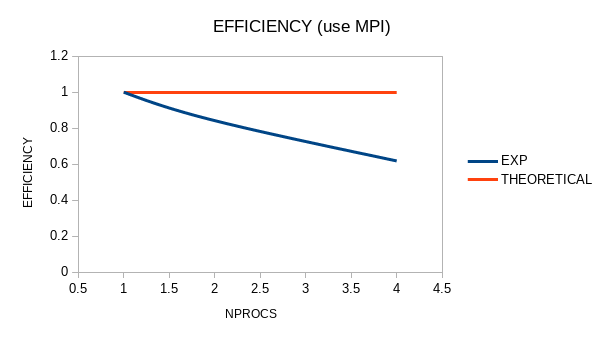
\includegraphics[height = 65mm,width = 140mm]{scaleMPIplot.png}   
        \caption{Scaling for mpi}                       
        \end{center}  
    \end{figure}   

    \newpage
    \section{CONCLUSION}

    \subsection{Speed up and ghost points}
    We can see from Figure 7 and 8 that although speedups are achieved, they are not that great. In fact, the experimental speedups are much lower than what we would expect. In terms of ghost points optimization, using 2 ghost points or 10 ghost points do not make a large difference. When using 10 ghost points, on some occasions such as using 8 and 10 cores, the results are worse than using 2 ghost points.  In order to investigate this thoroughly, I conduct ran the test again with smaller problem size (IMAX = 10) and then study the effects of ghost points and number of cores.  Figure 9 shows that for 1 core, we experience a very small window (between 1 and 2 ghost points) where we do have improvements.  However, after this, we do not see any improvements; in fact, it actually takes longer to run the code.  For 5 cores unde the same experiment, we can see that there are no improvements initially; however, as we increase the number of ghost points, we actually see speedup. I can then conclude that there is a sweet spot between problem size and number of cores which can help to improve the speedup.  In other words, for large problem size in Figure 7 and 8, the number of ghost points are not that great compare to the big problem size.  For 10,000 nodes, if I use 10 ghost points, then that only saves 10 iterations where the code does not have to perform any send/recv, this is insignificant.  For smaller problem size, 10 nodes, using 5 ghost points can save you 5 iterations which is basically half of the problem size.  Then, I tried to see if using 10,000 nodes and a significant number of ghost points can make any difference.  The results are as follow: 
    
    \begin{figure}[H]
        \centering
        \subfloat{{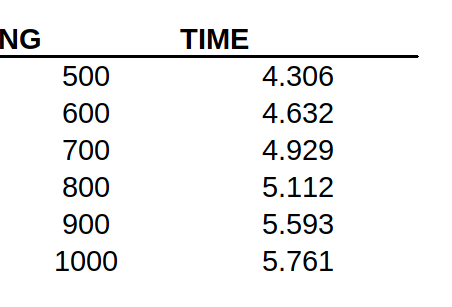
\includegraphics[width=5cm]{sigTable.png} }}%
        \qquad
        \subfloat{{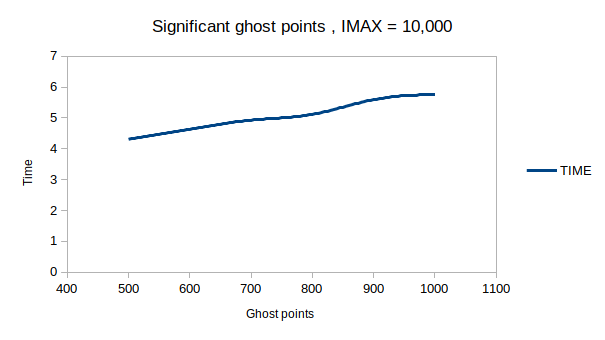
\includegraphics[width=12cm]{sigghost.png} }}%
        \caption{Significant ghost points for 10,000 nodes} 
    \end{figure}
    \noindent
    We do not see any improvements. The rationale here is that if a significant number of ghost points is used, then the code does not have to send/recv as much.  Although this is true, the problem is in how this code is constructed.  This prevents any speedup and will be discussed later on.  
    
    \subsection{MPI headers}
    It is interesting to note that the MPI header file to be used in Fortran, "mpif.h", is in fact said to be obsolette.  When running with the officially supported MPI header, we have better results in terms of scalability.  These are shown in Figure 10 and 11. Unfortunately, my laptop does not have more than 4 cores so we really can't make better conclusions regarding the MPI headers.

    \subsection{Remarks}
    \begin{itemize}
        \item Firstly, the code runs in parallel and we do see speedup; although these are not significant
        \item The ghost points optimization works but we need to do some more experiment to choose that sweet spot between problem size and number of ghost points. As of right now, there are no significant improvements. 
        \item Using more significant ghost points with bigger problem size seems to tbe the correct thinking; however, the current code advects the conservation of mass,momentum and energy together as 1 global vector U.  This is costly in terms of send/recv because we are actually sending and receiving a matrix of dimension 3 by number of ghost points. A better way to implement would be to advect the different conservation laws individually.  This would help when doing send/recv but we would need to figure out how compute the fluxes for mass, momentum and energy.     
    \end{itemize}

    \newpage
    \section{REFERENCES}
    \begin{enumerate}
        \item MTH/CSE 4082 Intro to Parallel Process lecture notes.  Dr. Jones Spring 2019. Florida Institute of Technology
        \item Chimrac CFD.  Web April 2019. \url{http://chimeracfd.com/programming/gryphon/fluxvanleer.html}
        \item Analytical Shocktube Python code. Web April 2019. \url{https://github.com/ibackus/sod-shocktube}
        \item Analytical Shocktube original source (referenced by the Github above). Web April 2019. Dr. Timmes. University of Arizona. \url{http://cococubed.asu.edu/code_pages/exact_riemann.shtml}
        
    \end{enumerate}

    \newpage
    \section{CODES}
    \subsection{Analytical Python Solver}
    \textbf{Note: The code below was taken to show the accuracy of the implementation. The author's work was cited in the the previous section.  These are not my own codes.}

    \lstinputlisting[language=Python,basicstyle=\fontsize{9}{11}\ttfamily]{sod.py}

    \newpage
    \subsection{Python Plotting}
    \textbf{I wrote this code on my own to use the analytical solver in previous section and the numerical results from my own implementation}

    \lstinputlisting[language=Python,basicstyle=\fontsize{9}{12}\ttfamily]{plotPYTHON.py}

    \newpage
    \subsection{1D Shocktube MPI Implementation}
    \textbf{Below is the main code for this project. This is my own work. Results are written to a file "result.txt". The python codes in previous sections are used to read and plotted along the analytical solutions}



    \lstinputlisting[basicstyle=\fontsize{9}{12}\ttfamily]{max_final.f90}



    
    

\end{document}